\documentclass[a4paper,12pt]{article}
\usepackage[utf8]{inputenc}
\usepackage[spanish]{babel}
\usepackage{tikz}
\usepackage{geometry}
\usepackage{setspace}
\usepackage{titlesec}
%\usepackage{lmodern}
\usepackage{multicol}
\usepackage{fancyhdr}
\usepackage{graphicx}
%\usepackage{helvet}
%\usepackage{mathptmx}
\usepackage{amsmath}       
\usepackage{amssymb}      
\usepackage{adjustbox}     
\usepackage{lastpage}
\usepackage{pgfplots}
\pgfplotsset{compat=1.17}
\usepackage{amsmath}
\usepackage{minted}
\usepackage{wrapfig}

\usepackage{tabularx}
\usepackage{qrcode}
\usepackage{tikz}
\usetikzlibrary{matrix, fit, positioning}

\usepackage{hyperref}
\usepackage{booktabs}
\usepackage{array}
\usepackage{float}
\usepackage{longtable}  

\renewcommand{\arraystretch}{1.4}
\setlength{\tabcolsep}{8pt} 

\setlength{\footskip}{25pt}
%---------------------------python
\usepackage[T1]{fontenc}
\usepackage[utf8]{inputenc}

\usepackage{listings}
\usepackage{xcolor}

\lstdefinestyle{pythonstyle}{
	language=Python,
	basicstyle=\ttfamily\small,
	keywordstyle=\color{blue},
	stringstyle=\color{red},
	commentstyle=\color{gray},
	numbers=left,
	numberstyle=\tiny\color{gray},
	stepnumber=1,
	numbersep=5pt,
	showspaces=false,
	showstringspaces=false,
	breaklines=true,
	frame=single,
	tabsize=4
}



%-------------------------------Consola
\usepackage{listings}
\usepackage{xcolor}

\lstdefinestyle{consola}{
	backgroundcolor=\color{black!5},
	basicstyle=\ttfamily,
	frame=single,
	keywordstyle=\color{blue},
	commentstyle=\color{gray},
	showstringspaces=false
}

%Plano Z y Z^2

\usepackage[utf8]{inputenc}
\usepackage{amsmath, amssymb}
\usepackage{pgfplots}
\pgfplotsset{compat=1.18}
\usepackage{geometry}
\geometry{a4paper, margin=2.5cm}


\geometry{top=2.5cm, bottom=2.5cm, left=2.5cm, right=1.5cm}

% Estilo de página
\pagestyle{fancy}
\fancypagestyle{miestilo}{
	\fancyhf{} % Limpia encabezado y pie
	
	% Encabezado izquierda: logo
	\fancyhead[L]{%
		\vspace{0.1cm}
		\adjustbox{valign=c,scale=0.15}{%
			\begin{tikzpicture}
				\clip (-3,-2.8) rectangle (3,2.8);
				\draw[black,line width=0.8cm] (-2.3,0)--(2.3,0);
				\draw[black,line width=0.8cm] (0,-2.85)--(0,2.85);
				\draw[black,line width=0.87cm] (0,2.8) circle(2);
				\draw[black,line width=0.87cm] (0,-2.8) circle(2);
			\end{tikzpicture}
		}%
	}
	
	% Encabezado centro: título
	\fancyhead[C]{\textbf{Técnicas Digitales 1   
	}}
	
	% Encabezado derecha: TP y año debajo
	\fancyhead[R]{%
		Ejercicio 5 \\ 2026
	}
	
	% Línea en el encabezado y pie
	\renewcommand{\headrulewidth}{0.4pt}
	\renewcommand{\footrulewidth}{0.4pt}
	
	% Pie de página derecha: Página X de Y
	\fancyfoot[R]{Página \thepage\ de \pageref{LastPage}}
}


\begin{document}
	
	% --------- PORTADA ---------
	\pagestyle{empty}
	\begin{center}
		\textbf{\LARGE UNIVERSIDAD TECNOLÓGICA NACIONAL}\\[0.2cm]
		\textbf{\Large FACULTAD REGIONAL CÓRDOBA}\\[0.5cm]
		\textbf{\large INGENIERÍA ELECTRÓNICA}\\[1.5cm]
		
		\begin{tikzpicture}
			\clip (-3,-2.8) rectangle (3,2.8);
			\draw[black,line width=0.8cm] (-2.3,0)--(2.3,0);
			\draw[black,line width=0.8cm] (0,-2.85)--(0,2.85);
			\draw[black,line width=0.87cm] (0,2.8) circle(2);
			\draw[black,line width=0.87cm] (0,-2.8) circle(2);
		\end{tikzpicture}
		
		\vspace{1cm}
		\textbf{\huge Técnicas Digitales 1   
		}\\[0.5cm]
		\rule{\textwidth}{0.4pt}\\[0.3cm]
		\textbf{\Huge Actividad Práctica – Ejercicio 5 (Meses de 31 días)
		}\\[0.3cm]
		{\large Implementación en Verilog}\\[0.3cm]
		\rule{\textwidth}{0.4pt}\\[1.5cm]
	\end{center}
	
	\begin{flushleft}
		\begin{tabular}{@{}ll}
			DOCENTES     & : Esp.Ing. Marcelo Casasnovas\\ 
			& \ \  Ing Florencia Belén Molla JTP \\[0.2cm]
			CÁTEDRA      & :  Técnicas Digitales 1   \\[0.2cm]
			CURSO        & : 3R4 \\[0.2cm]
			ALUMNO      & :
			\begin{tabular}[t]{@{}l l}
				Gonza Elías Noel Imanol           & 87669 \\ 
			\end{tabular}
		\end{tabular}
	\end{flushleft}
	
	\vfill
	\begin{center}
		\textbf{CÓRDOBA, ARGENTINA}\\
		\textbf{2026}
	\end{center}
	\pagestyle{empty}
	% --------- CAMBIO DE ESTILO ---------
	\newpage
	\pagenumbering{arabic}
	\pagestyle{miestilo}
	% --------- CONTENIDO ---------
	\tableofcontents
	\newpage
	

	\section*{Ejercicio 5: Meses de 31 días}
	
	Se desea diseñar un circuito lógico que determine si un mes posee 31 días. 
	Para representar los meses se utiliza una entrada binaria de 4 bits:
	
	\[
	A_3A_2A_1A_0
	\]
	
	La salida será:
	
	\[
	T =
	\begin{cases}
		1, & \text{si el mes posee 31 días} \\
		0, & \text{si el mes no posee 31 días}
	\end{cases}
	\]
	
	Los meses que poseen 31 días son:
	
	\[
	1,\ 3,\ 5,\ 7,\ 8,\ 10,\ 12
	\]
	
	Los valores que no corresponden a ningún mes, es decir del 13 al 15, se toman como condiciones de no importa.
	
	\[
	13,\ 14,\ 15 = X
	\]
	
	\subsection*{Tabla de verdad}
	
	\begin{table}[h!]
		\centering
		\begin{tabular}{|c c c c|c|c|}
			\hline
			$A_3$ & $A_2$ & $A_1$ & $A_0$ & Mes & $T$ \\
			\hline
			0 & 0 & 0 & 0 & 0  & X \\
			0 & 0 & 0 & 1 & 1  & 1 \\
			0 & 0 & 1 & 0 & 2  & 0 \\
			0 & 0 & 1 & 1 & 3  & 1 \\
			0 & 1 & 0 & 0 & 4  & 0 \\
			0 & 1 & 0 & 1 & 5  & 1 \\
			0 & 1 & 1 & 0 & 6  & 0 \\
			0 & 1 & 1 & 1 & 7  & 1 \\
			1 & 0 & 0 & 0 & 8  & 1 \\
			1 & 0 & 0 & 1 & 9  & 0 \\
			1 & 0 & 1 & 0 & 10 & 1 \\
			1 & 0 & 1 & 1 & 11 & 0 \\
			1 & 1 & 0 & 0 & 12 & 1 \\
			1 & 1 & 0 & 1 & 13 & X \\
			1 & 1 & 1 & 0 & 14 & X \\
			1 & 1 & 1 & 1 & 15 & X \\
			\hline
		\end{tabular}
		\caption{Tabla de verdad para determinar los meses de 31 días.}
	\end{table}
	
	\subsection*{Mapa de Karnaugh}
	
	El mapa de Karnaugh se arma considerando las variables $A_3A_2$ en las filas y $A_1A_0$ en las columnas.
	
\[
\begin{tikzpicture}
	
	\matrix (K) [
	matrix of nodes,
	nodes={
		draw,
		minimum width=1.2cm,
		minimum height=0.8cm,
		anchor=center
	},
	column sep=-\pgflinewidth,
	row sep=-\pgflinewidth
	] {
		& 00 & 01 & 11 & 10 \\
		00     & X  & 1  & 1  & 0  \\
		01     & 0  & 1  & 1  & 0  \\
		11     & 1  & X  & X  & X  \\
		10     & 1  & 0  & 0  & 1  \\
	};
	
	% Etiquetas
	\node[left=0.3cm of K-3-1] {$A_3A_2$};
	\node[above=0.3cm of K-1-3] {$A_1A_0$};
	
	% Grupo central cerrado
	\node[
	draw=red,
	rounded corners,
	very thick,
	inner sep=3pt,
	fit=(K-2-3)(K-2-4)(K-3-3)(K-3-4)
	] {};
	
	% Grupo lateral izquierdo cortado
	\draw[violet, very thick]
	([xshift=-0.1cm,yshift=0.1cm]K-4-2.north west) --
	([xshift=0.1cm,yshift=0.1cm]K-4-2.north east) --
	([xshift=0.1cm,yshift=-0.1cm]K-5-2.south east) --
	([xshift=-0.1cm,yshift=-0.1cm]K-5-2.south west);
	
	% Grupo lateral derecho cortado
	\draw[violet, very thick]
	([xshift=0.1cm,yshift=0.1cm]K-4-5.north east) --
	([xshift=-0.1cm,yshift=0.1cm]K-4-5.north west) --
	([xshift=-0.1cm,yshift=-0.1cm]K-5-5.south west) --
	([xshift=0.1cm,yshift=-0.1cm]K-5-5.south east);
	
\end{tikzpicture}
\]

	
	\subsection*{Simplificación}
	
	A partir del mapa de Karnaugh se obtienen los siguientes grupos:
	
	\[
	T = \overline{A_3}A_0 + A_3\overline{A_0}
	\]
	
	Esta expresión corresponde a una compuerta XOR entre $A_3$ y $A_0$:
	
	\[
	\boxed{T = A_3 \oplus A_0}
	\]
	
	Por lo tanto, la función lógica simplificada queda:
	
	\[
	\boxed{T = A_3 \oplus A_0}
	\]
	
\section{Implementación y simulación en ISE Xilinx}

A partir de la función lógica simplificada mediante el mapa de Karnaugh:

\[
T = A_3 \oplus A_0
\]

se realizó la implementación del circuito en lenguaje Verilog utilizando el entorno ISE Xilinx. La salida $T$ indica si el mes ingresado posee 31 días.

\subsection{Código Verilog del módulo principal}

En la Figura \ref{fig:verilog-modulo} se muestra el código Verilog correspondiente al módulo principal. En este se declaran las entradas $A_3$, $A_2$, $A_1$, $A_0$ y la salida $T$. La operación lógica se implementa mediante el operador XOR.

\begin{figure}[H]
	\centering
	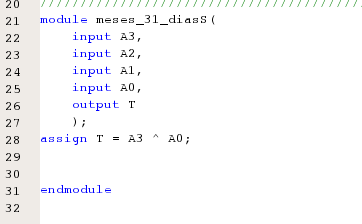
\includegraphics[width=0.5\textwidth]{verilog_modulo.png}
	\caption{Código Verilog del módulo principal.}
	\label{fig:verilog-modulo}
\end{figure}

\subsection{RTL generado}

Luego de sintetizar el módulo en ISE Xilinx, se generó el esquema RTL del circuito. En la Figura \ref{fig:rtl} se observa que la función lógica obtenida se implementa mediante una compuerta XOR, lo cual coincide con la expresión simplificada.

\begin{figure}[H]
	\centering
	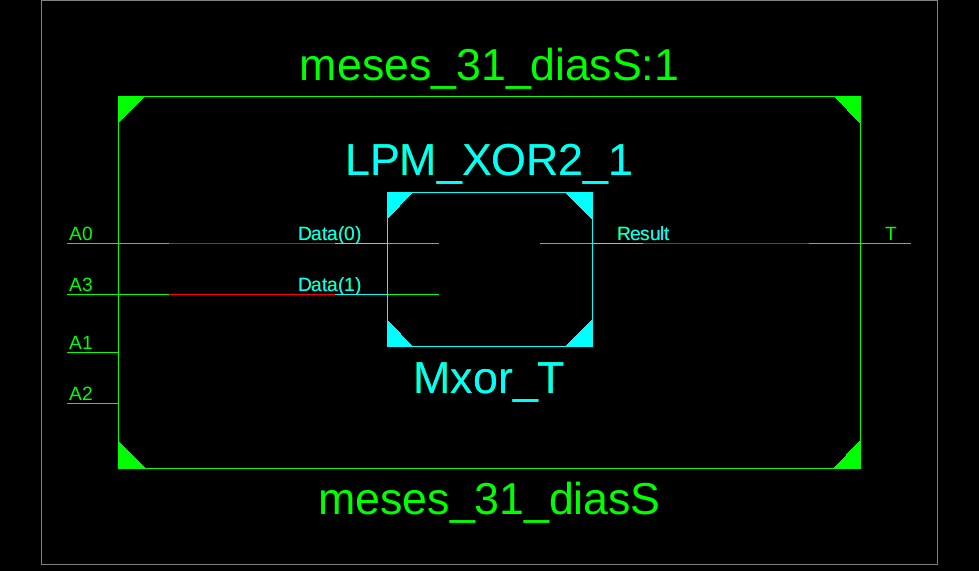
\includegraphics[width=0.5\textwidth]{rtl_schematic.png}
	\caption{Esquema RTL generado en ISE Xilinx.}
	\label{fig:rtl}
\end{figure}

\subsection{Código Verilog del testbench}

Para verificar el funcionamiento del circuito se realizó un archivo de prueba o \textit{testbench}. En este se simularon los valores binarios correspondientes a los meses del 0 al 12, observando el valor de salida $T$ para cada caso.

\begin{figure}[H]
	\centering
	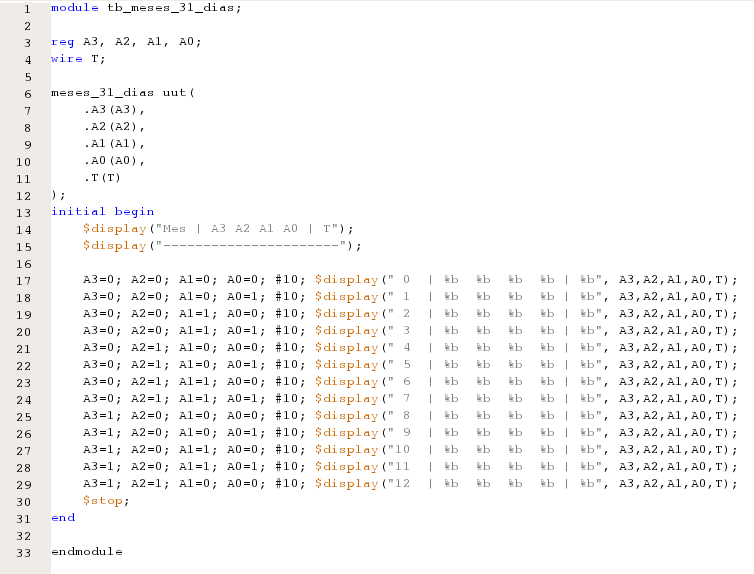
\includegraphics[width=0.85\textwidth]{verilog_testbench.png}
	\caption{Código Verilog del testbench utilizado para la simulación.}
	\label{fig:testbench}
\end{figure}

\subsection{Resultado de la simulación}

En la Figura \ref{fig:consola} se muestra el resultado obtenido en la consola de ISim. La salida $T$ toma el valor lógico 1 para los meses que poseen 31 días y el valor lógico 0 para los meses que no poseen 31 días.

\begin{figure}[H]
	\centering
	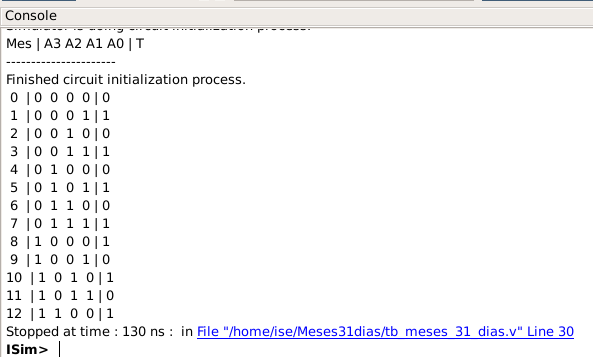
\includegraphics[width=0.7\textwidth]{consola_simulacion.png}
	\caption{Resultado de la simulación en la consola de ISim.}
	\label{fig:consola}
\end{figure}
	


	\subsection*{Conclusión}
	
	Mediante la tabla de verdad y la simplificación por mapa de Karnaugh, se determinó que la salida $T$ depende únicamente de las variables $A_3$ y $A_0$. 
	Por lo tanto, el circuito puede implementarse utilizando una sola compuerta XOR.

\begin{figure}[h]
	\centering
	\qrcode[height=4cm]{https://github.com/Enig17/TecnicasDigitales1/blob/0e1d32dfd12a191127b5900767db057132379c51/Ejercicio%205/Ejercicio5.pdf}
	\vspace{0.3cm}
	
	\url{https://github.com/Enig17/TecnicasDigitales1/blob/0e1d32dfd12a191127b5900767db057132379c51/Ejercicio%205/Ejercicio5.pdf}
	\caption{Repositorio del informe en GitHub}
\end{figure}
\end{document}